\section{H$\infty$-Regler}
\begin{itemize}
	\item Wenn die Regelstrecke nicht exakt bekannt ist, oder sich mit der Zeit verändern kann
	\item Kompensieren einer Abweichung zum theoretisch entworfenem Regler
	\begin{itemize}
		\item Dabei stellt $\Delta$ die Abweichung zur theoretisch ermittelten Strecke dar. 
		\item Eine andere Bezeichnung für $\Delta$ ist Modellunsicherheit
	\end{itemize}
	\item $P_0$ bezeichnet die nominale Regelstrecke
\end{itemize}
\begin{figure}[h!]
	\centering
	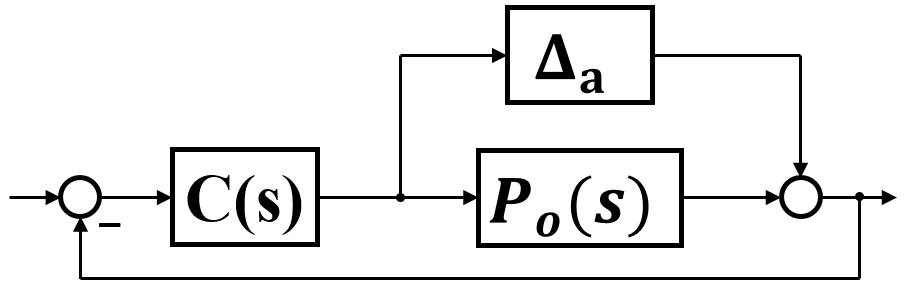
\includegraphics[width=0.25\linewidth]{bilder/HInf1}
	\label{fig:hinf1}
\end{figure}

\subsection{Basics}
\begin{itemize}
	\item Die H$\infty$-Norm ist der höchste Punkt im Bode-Diagramm der zu untersuchenden Funktion
	\item $\text{H}_\infty\text{-Norm} = \lVert P(s) \rVert_\infty$
	\begin{itemize}
		\item In untenstehender Abbildung ist ein Beispiel gezeigt. Die $\text{H}_\infty\text{-Norm}$ ist für diese Funktion $A$
	\end{itemize}
	\item Die Robuste Regelung funktioniert bei den klassischen Stabilitätsbeobachtung (Phasen- und Amplitudenreserve)
	\begin{itemize}
		\item Es gibt keine analytische Optimierungsmethode
		\item Auch bei scheinbarer Stabilität (durch übliche Kriterien) ist diese keine Garantie für Stabilität des Regelkreise. 
	\end{itemize}
\end{itemize}

\begin{figure}[!ht]
	\centering
	\subfloat[$\text{A}=\lVert H \rVert_\infty$ von $G(s)$ \label{subfig:hinf1}]{
		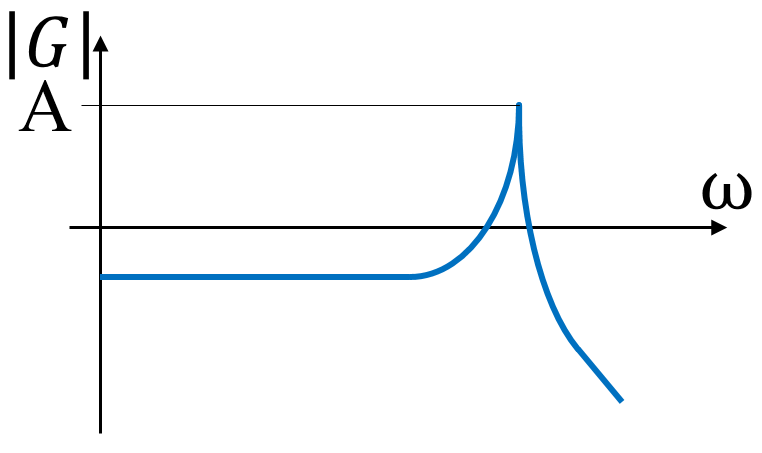
\includegraphics[width=0.25\textwidth]{./bilder/HInf2.PNG}
	}
	\subfloat[Additive Modellunsicherheit \label{subfig:hinf2}]{
		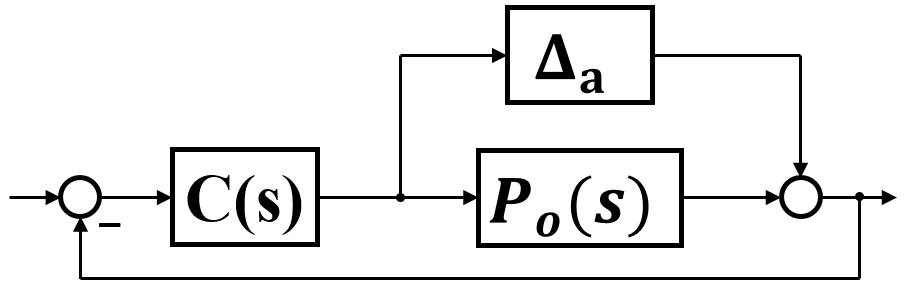
\includegraphics[width=0.25\textwidth]{./bilder/HInf1.PNG}
	}
	\subfloat[Multiplikative Modellunsicherheit \label{subfig:hinf3}]{
		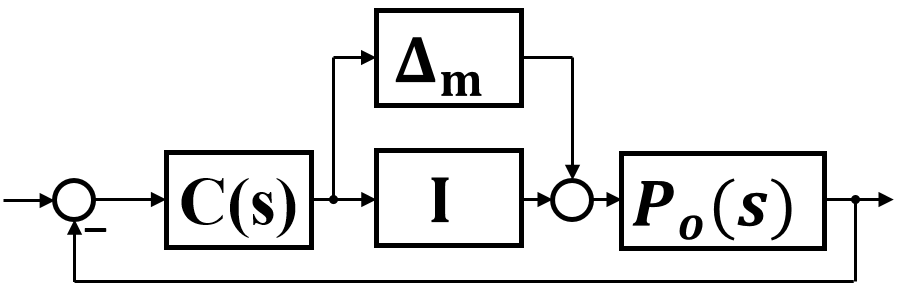
\includegraphics[width=0.25\textwidth]{./bilder/HInf3.PNG}
	}\\
	\label{fig:hinf2}
\end{figure}

\subsection{Staibiltätsanalyse $\rightarrow$ Small-Gain-Theorem}
\subsubsection{Additive Modellunsicherheit}
\begin{itemize}
	\item Modell kann umgezeichnet werden wie in unterstehender Abbildung \ref{subfig:hinf4} gezeigt
	\item In Gleichung \ref{eq:defAddUnsicherheit} ist die Formel für die additive Unsicherheit gezeigt
	\item In Gleichung \ref{eq:addStabilitaet} ist das Kriterium für die Stabilität bei additiver Modellunsicherheit gezeigt
	\item Additive Unsicherheiten können im Nyquist-Diagramm visualisiert werden (siehe Abbildung 9, Skript s.16)
\end{itemize}
\begin{align}
	\label{eq:defAddUnsicherheit}
	\Delta_a(s) &= P(s)-P_0(s)\\
	\label{eq:addStabilitaet}
	\lVert\Delta_a\rVert_\infty &< \frac{1}{\left\lVert\frac{C}{1+P_0C}\right\rVert_\infty} \qquad \Delta_a(s) = P(s)-P_0(s)
\end{align}

\subsubsection{Multiplikative Modellunsicherheit}
\begin{itemize}
	\item Modell kann umgezeichnet werden wie in unterstehender Abbildung \ref{subfig:hinf6} gezeigt
	\item In Gleichung \ref{eq:defMulUnsicherheit} ist die Formel für die Multiplikative Unsicherheit gezeigt
	\item In Gleichung \ref{eq:mulStabilitaet} ist das Kriterium für die Stabilität bei multiplikativer Modellunsicherheit gezeigt
	\item Multiplikative Unsicherheiten können gut in einem Bode-Diagramm dargestellt werden (siehe Abbildung 9, Skript s.16)
\end{itemize}
\begin{align}
\label{eq:defMulUnsicherheit}
\Delta_m(s) &= \frac{P(s)}{P_0(s)}-1\\
\label{eq:mulStabilitaet}
\lVert\Delta_m\rVert_\infty &< \frac{1}{\left\lVert\frac{P_0C}{1+P_0C}\right\rVert_\infty} \qquad 
\end{align}

\begin{figure}[!h]
	\centering
	\subfloat[Modell der additiven Unsicherheit \label{subfig:hinf4}]{
		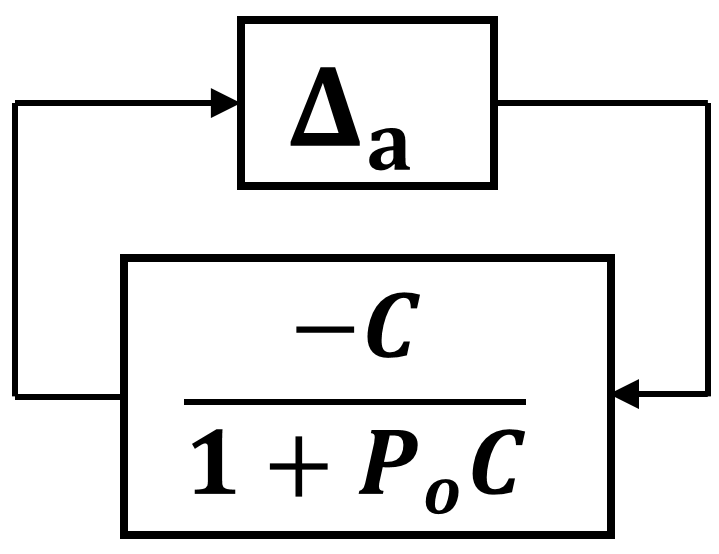
\includegraphics[width=0.15\textwidth]{./bilder/HInf4.PNG}
	}\hspace{0.2\linewidth}
	\subfloat[Modell der multiplikativen Unsicherhei \label{subfig:hinf6}]{
		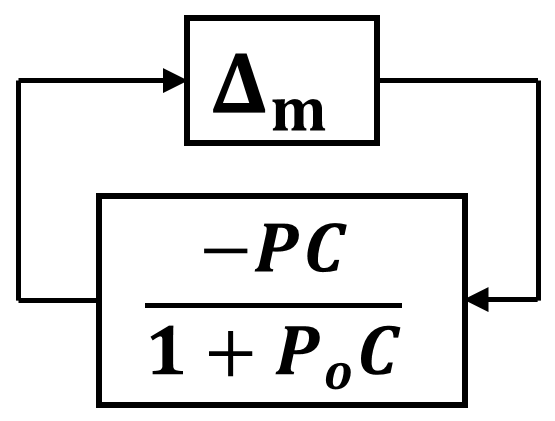
\includegraphics[width=0.15\textwidth]{./bilder/HInf6.PNG}
	}\\
	\caption{ $\text{H}_\infty$-Regelkreise in anderer Darstellung}
	\label{fig:hinf4}
\end{figure}


\subsection{Regelgüte}

\begin{itemize}
	\item Die Funktionen $w_1$, $w_{2a}$ und $w_{2m}$ dürfen nicht mit einem Integrator oder Differentiator beginnen!
	\item Damit dies verhindert wird, werden die Terme $\frac{1}{s}$ resp. $s$ ersetzen durch einen Sehr schnellen Tief-, resp. Hochpass, siehe nachfolgendes Beispiel.
	\item Damit werden Probleme in Berechnung bei $s=0$ verhindert und korrigierte Funktion befriedigt Kriterien für Stabilität
	\item Für die Regelgüte müssen die Gleichungen \ref{eq:GueteAdditiv} und \ref{eq:GueteMultiplikativ} erfüllt sein 
\end{itemize}
\begin{align}
	\label{eq:GueteAdditiv}
	\left\lVert w_{2a}  \frac{C}{1+PC}\right\rVert_\infty < 1\\
	\label{eq:GueteMultiplikativ}
	\left\lVert w_{2m} \frac{PC}{1+PC}\right\rVert_\infty<1
\end{align}

\begin{figure}[!h]
	\centering
	\subfloat[Modell für die Regelgüte mit allen verwendeten Grössen \label{subfig:hinf8}]{
		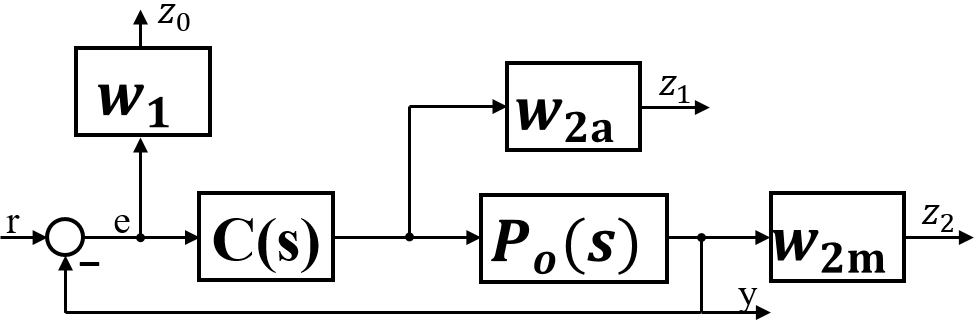
\includegraphics[width=0.35\linewidth]{./bilder/HInf8.PNG}
	}\quad
	\subfloat[Kritische Distanz im Nyquist-Diagramm \label{subfig:hinf7}]{
		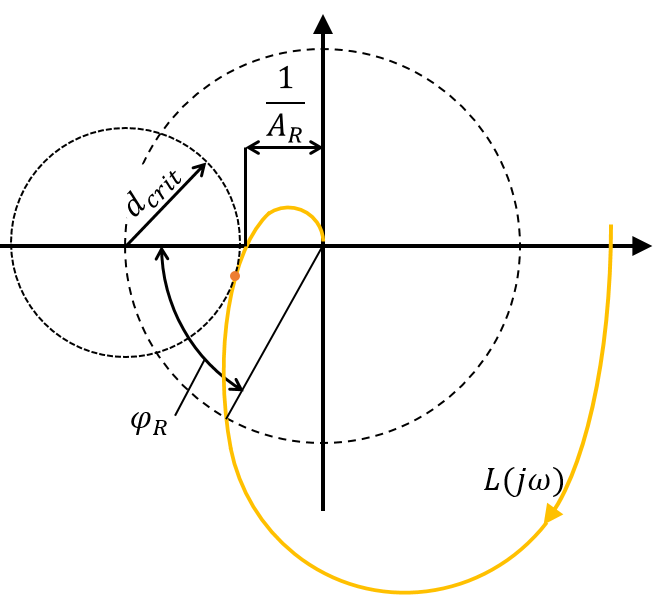
\includegraphics[width=0.27\linewidth]{./bilder/HInf7.PNG}
	}\quad
	\subfloat[Amplitudengang von $S$ und $w_1$  \label{subfig:hinf9}]{
		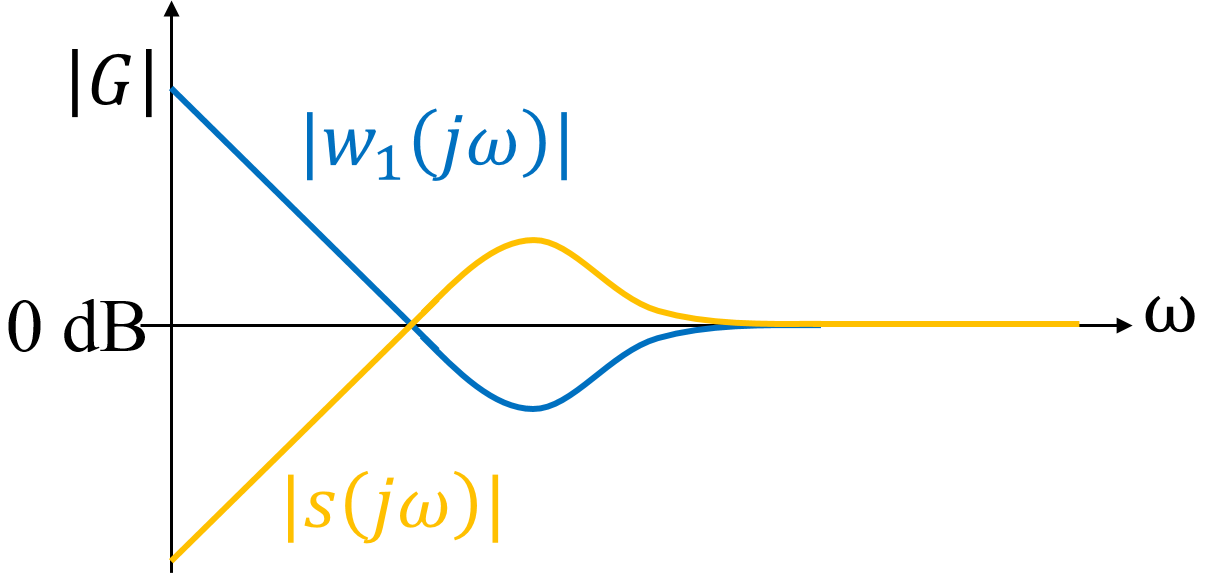
\includegraphics[width=0.27\linewidth]{./bilder/HInf9.PNG}
	}
	\caption{Verschiedene Bilder zu Regelgüte und Senitivitätsfunktion}
	\label{fig:hinf7}
\end{figure}

\begin{tabularx}{\linewidth}{p{0.5\linewidth} p{0.5\linewidth}}
	\textbf{Integrator } bei $\omega=0$	&\textbf{Differentiatior} bei $\omega=0$		\\
	%Zeile 2 mit Allen Bildern
	\includegraphics[width=.5\linewidth]{bilder/hinf12}&
	\includegraphics[width=.5\linewidth]{bilder/hinf11}\\
	%Zeile 2
	%Zeile 3 Mit den Formeln
	\begin{equation*}
	w_1(s) =\frac{1}{s} \quad\Rightarrow w_1(s) = \frac{1}{s+10^{-5}}
	\end{equation*}&
	\begin{align*}
	w_{2a}=\frac{7.5s}{(s+1)(s+15)}\quad\Rightarrow w_{2a} = \frac{0.0075s(s+1000)}{(s+1)(s+15)}
	\end{align*}
\end{tabularx}


\subsubsection{Sensitivitätsfunktion}
\begin{itemize}
	\item $S=$ Sensitivität entspricht dem Übergang von $r$ auf $e$ oder von $d$ auf $y$
	\item Die kritische Distanz maximieren geht einher mit dem Minimieren der $\lVert\text{S}\rVert_\infty$
	\item Erinnerung: $L(s) = P(s)\cdot C(s)$ und wird im open-Loop eingetragen
	\item Robuste Regler zielen darauf ab die kritische Distanz zu maximieren (also $\lVert S \rVert_\infty$ zu minimieren
%?	\item Wird der Amplitudengang von $S(j\omega)$ an der 0-dB-Linie gespiegelt gibt sich gerade der Amplitudengang von $w_1(j\omega)$
	\item Die Funktion $w_1$ ist eine Gewichtungsfunktion (siehe Abbildung \ref{subfig:hinf8}).
	\begin{itemize}
		\item Bei einer Resonanz von $S$ bei $w_1$ eine Zusätzliche Polstelle bei der ca. doppelten Resonanzfrequenz einführen
	\end{itemize}
	\item Die Bode Integralrelation besagt, dass für die Sensitivitätsfunktion die Fläche unterhalb der 0 dB-Linie gleich sein muss wie die Fläche oberhalb der 0 dB-Linie. 
	\begin{itemize}
		\item [\textbf{Achtung:}] Das Flächenverhältnis muss identisch sein, wenn $\omega$ nicht logarithmisch dargestellt wird!
		\item Gezeigt in Abbildung \ref{fig:hinf10}
		\item Je höher (und dadurch kürzer) die orange Fläche ist, desto schneller wird der Regler. Diese Geschwindigkeit geht auf kosten der Stabilität.
	\end{itemize}
\end{itemize}
\begin{align*}
	d_\text{crit}&= \frac{1}{\lVert S \rVert_\infty} \qquad \text{ und } \qquad S(j\omega)=\frac{1}{1+L(J\omega)} = \frac{1}{1+P(j\omega)\cdot C(j\omega)}\\
	T(s) &= \frac{L(s)}{1+L(s)}
\end{align*}
\begin{figure}[!h]
	\centering
	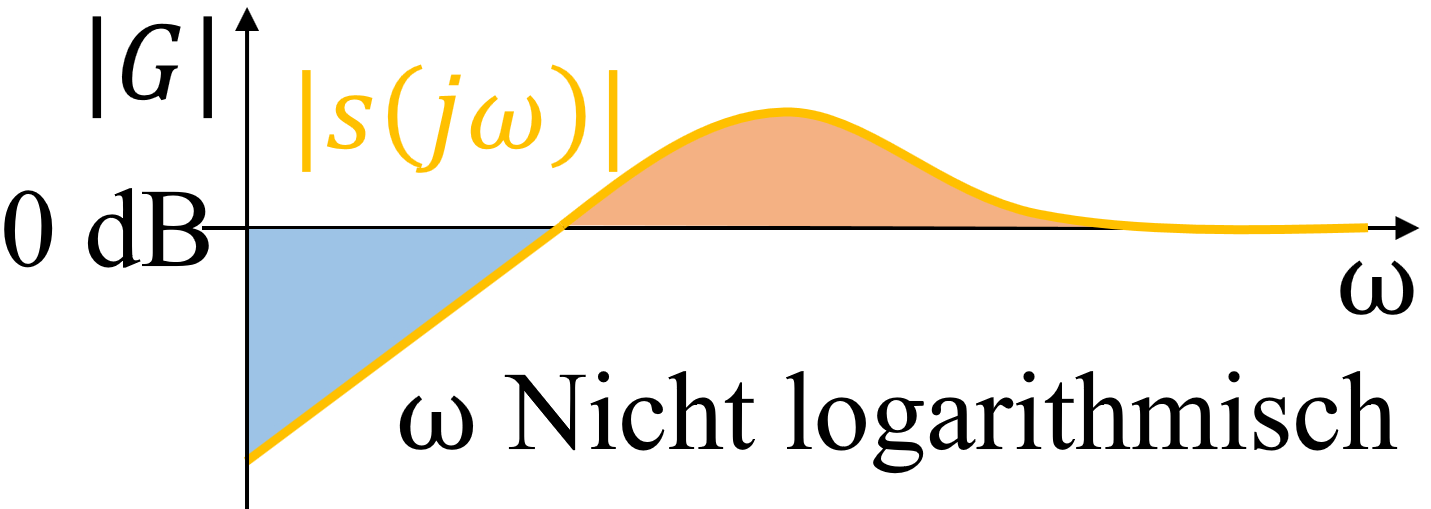
\includegraphics[width=0.2\linewidth]{bilder/HInf10}
	\caption{Trade-Off zwischen Stabilität und Geschwindigkeit}
	\label{fig:hinf10}
\end{figure}

\subsubsection{Gemischter Senitivitätsanspruch}
\begin{itemize}
	\item Funktion soll sowohl Sensitivität des Fehlers, wie auch die additive, oder multiplikative Unsicherheit berücksichtigen
	\item Die Matrix entspricht der Übertragung von $r$ nach $z$
	\item Für Additive Modellunsicherheit Formel \ref{eq:mixedApproachAdd}
	\item Für Multiplikative Modellunsicherheit Formel \ref{eq:mixedApproachMul}
\end{itemize}
\begin{align}
	\label{eq:mixedApproachAdd}
	\left\lVert\begin{bmatrix}
		w_1\frac{1}{1+PC}\\
		w_{2a}\frac{C}{1+PC}
	\end{bmatrix}\right\rVert_\infty <1 \qquad \text{Übertragungsfunktion von }r\text{ nach } \begin{bmatrix}
		z_0\\z_1
	\end{bmatrix}\\
		\label{eq:mixedApproachMul}
	\left\lVert\begin{bmatrix}
	w_1\frac{1}{1+PC}\\
	w_{2m}\frac{PC}{1+PC}
	\end{bmatrix}\right\rVert_\infty <1 \qquad \text{Übertragungsfunktion von }r\text{ nach } \begin{bmatrix}
	z_0\\z_2
	\end{bmatrix}
\end{align}

\subsection{Linear Fractional Transformation (LFT)}
\begin{itemize}
	\item Die LFT von $P$ und $\Delta$ wird geschrieben als $\mathcal{F}\left(P,\Delta\right)$
	\item Für ein SISO-System ist es eine bilineare Transofrmation
	\item Eingänge von Ausserhalb nur in $P$ einführen, falls nötig hindruch passieren mit einer Einheitsmatrix
	\item Entgegen der Abbildung können auch mehrere Eingänge hinein kommen
	\item Beim Umschreiben eines Systems zum LFT alle $P_i$ und alle $C_i$ zusammenfassen
	\item Vorgehen zum erstellen der Matrix $P$
	\begin{itemize}
		\item Achtung: Dieses Vorgehen ist nur sinngemäss beschrieben, aus Zeitgründen und fehlendem Verständnis, wird diese Zusammenfassung hier gewisse Fehler aufweisen. 
		\item [1.] In System in klassischer Schreibweise: Boxen um die zusammenzufassenden Blöcke zeichnen (Systemgrenzen bestimmen)
		\item [2.] Ein- und Ausgänge definieren 
		\item [3.] Alles was in das System von Aussen kommt muss über Block $P$ eingespiesen werden
		\item [4.] $\dot{x} = Px$ wobei $\dot{x}$ dem nächsten Schritt entspricht (analog dem Aufbau der Matrix $A$ )
	\end{itemize}
	\item Beispiel siehe Beispiel unten (entsprechend der Aufgabe 1 von \glqq Robust Control \grqq)
\end{itemize}


\begin{figure}[h!]
	\centering
	\begin{minipage}{0.25\linewidth}
		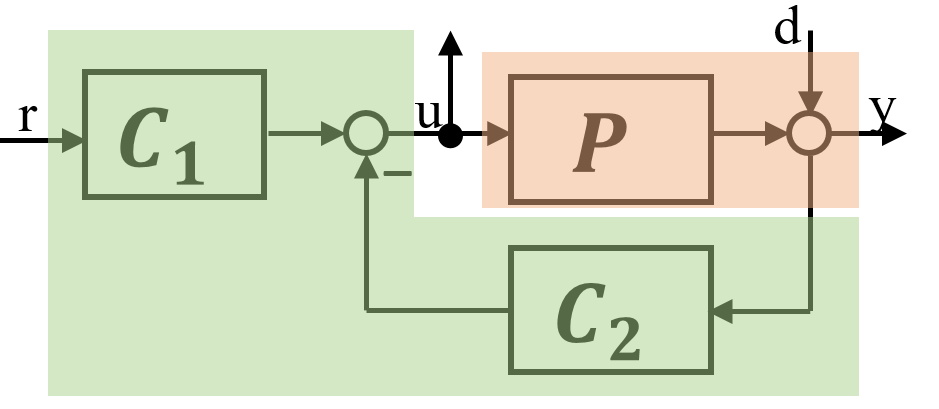
\includegraphics[width=1\linewidth]{bilder/LFT3}
	\end{minipage}
	\begin{minipage}{0.25\linewidth}
		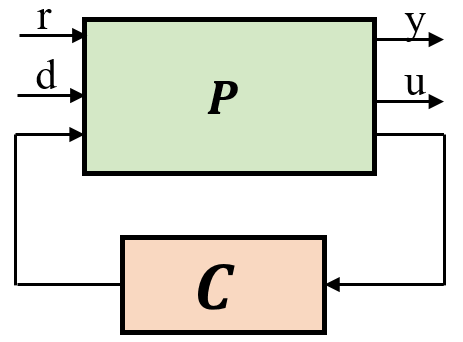
\includegraphics[width=.75\linewidth]{bilder/LFT4}
	\end{minipage}
	\begin{minipage}{0.45\linewidth}
		\footnotesize
			\begin{equation*}
		C: u = \begin{bmatrix}
		C_1 & -C_2
		\end{bmatrix} \begin{bmatrix}
		r\\y
		\end{bmatrix}				
		\end{equation*}
		\begin{equation*}
		\begin{bmatrix}
		y\\u\\y\\r
		\end{bmatrix} = \begin{bmatrix}
		0 & I & P\\
		0 & 0 & I\\
		I & 0 & 0\\
		0 & I & P
		\end{bmatrix}\begin{bmatrix}
		r\\d\\u
		\end{bmatrix}
		\end{equation*}
	\end{minipage}
\end{figure}

\begin{figure}[!h]
	\begin{minipage}{0.25\linewidth}
		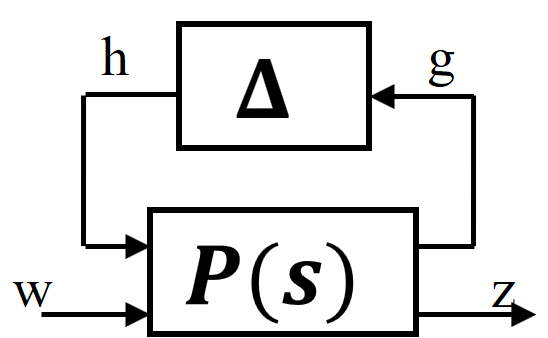
\includegraphics[width=.75\linewidth]{bilder/LFT1}
	\end{minipage}
	\begin{minipage}{0.35\linewidth}
		\footnotesize
		\textbf{Additive Modellunsicherheit}
		\begin{equation*}
			P = \begin{bmatrix}
				0 	& I\\
				I	& P_0
			\end{bmatrix}
		\end{equation*}
	\end{minipage}
	\begin{minipage}{0.35\linewidth}
		\footnotesize
		\textbf{Multiplikative Modellunsicherheit}
		\begin{equation*}
			P = \begin{bmatrix}
				0 	& P_0\\
				I	& P_0
			\end{bmatrix}
		\end{equation*}
	\end{minipage}
\end{figure}
\newpage